% 原书 p.231–p.237（PDF p.239–p.245）
% 第 9 章 9.1 节：更多例子

\chapter{拉格朗日子的硬故事（Hard Stories on Lagrangians）}

% >>> p239
回忆我们已在 1.6 节学习了拉格朗日子流形的基本定义与性质。此外，2.8 节中的定理 2.8.1
（Arnold--Liouville 定理）断言：环面作用会诱导出大量拉格朗日子流形（更确切地说，是环面）。
本章我们将进一步发展研究拉格朗日子流形的理论。关于本章标题中的「硬」（hard）一词：
按照 Gromov 的分类，辛几何中的问题分为硬问题与软问题。Hard 意为 obstruction（障碍），
通常描述辛几何中对象的不变性质。硬问题的研究往往基于 $J$-全纯曲线（例如 5.4 节介绍的
哈密顿 Floer 理论，它是哈密顿微分同胚的一个不变量）。Soft 意为 flexibility（柔性），
主要基于 [100, 51] 中发展的 h-原理（h-principle，其中 h 简写自 homotopy）。软问题的研究
通常旨在确认一个对象在某种形变下与另一个对象大致相同。这常常在辛几何与切触几何中给出
令人惊讶的结果（见 [31]），但遗憾的是，受篇幅所限，本书不涉及 h-原理的任何专题。
完整的介绍与处理见 [51]。
% [Tutor Note: 原文疑误——原文 \"provides surprisingly results\" 中 surprisingly 应为
% surprising（形容词修饰 results）。译文按正确含义处理，详见 qsg/notes/review_ch09a.md。]

\section{更多例子（More Examples）}

\begin{keytakeaways}
\begin{itemize}
  \item 几何图像：在 $S^2\times S^2$ 中至少可构造三个拉格朗日环面——Clifford 环面
        $\mathbb{T}_{\mathrm{Clifford}}$、Entov--Polterovich 环面
        $\mathbb{T}_{\mathrm{EP}}$ 与 Chekanov--Schlenk 环面 $\mathbb{T}_{\mathrm{CS}}$；
        前两者不同构，后两者辛同构。
  \item 数学工具：Arnold--Liouville 定理、Poisson 交换函数、$S^2$ 上的面积形式
        $\omega_{S^2}(v,w)=\langle p,v\times w\rangle$、旋转矩阵 $R_s$ 与环面作用的复合。
  \item 本节结论：定理 9.1.1（$\mathbb{T}_{\mathrm{EP}}\simeq\mathbb{T}_{\mathrm{CS}}$）
        与定理 9.1.2（$\mathbb{T}_{\mathrm{Clifford}}\not\simeq\mathbb{T}_{\mathrm{EP}}$，
        后者需借助下一节的 $A_\infty$-代数与势函数来证明）。
\end{itemize}
\end{keytakeaways}

考虑辛流形 $S^2\times S^2$，赋予乘积辛结构
$\omega_{\mathrm{prod}}=\pi_1^*\omega_{S^2}+\pi_2^*\omega_{S^2}$，其中 $\omega_{S^2}$ 由
(9.3) 定义，$\pi_i\colon S^2\times S^2\to S^2$（$i=1,2$）是投影映射。我们将介绍三个
拉格朗日环面。

\textbf{环面一：}考虑 $S^1\times S^1$，其中两个 $S^1$ 都是 $S^2$ 的标准赤道。则它是一个
拓扑环面，记作 $\mathbb{T}_{\mathrm{Clifford}}$，称为 $(S^2\times S^2,\omega_{\mathrm{prod}})$
中的\textbf{Clifford 环面}。

\textbf{环面二：}把 $S^2$ 等同于 $\R^3$ 的子集，定义为
\begin{equation}\tag{9.1}
  S^2=\bigl\{v=(v_1,v_2,v_3)\in\R^3\bigm| |v|^2=v_1^2+v_2^2+v_3^2=1\bigr\}.
\end{equation}
% >>> p240
于是 $S^2\times S^2\subset\R^3\times\R^3$。考虑如下定义的子集
$\mathbb{T}_{\mathrm{EP}}$：
\begin{equation}\tag{9.2}
  \mathbb{T}_{\mathrm{EP}}:=\bigl\{(v,w)\in S^2\times S^2\bigm|
  v_1+w_1=0,\ v\cdot w=-\tfrac12\bigr\},
\end{equation}
其中 $v\cdot w$ 是 $\R^3$ 中向量 $v$ 与 $w$ 的点积。我们断言
$\mathbb{T}_{\mathrm{EP}}$ 是 $S^2\times S^2$ 中的拉格朗日环面。这里「EP」代表
Entov--Polterovich，因为这个环面是在 [79] 的例 1.20 中引入并研究的。

乍一看，要验证 $\mathbb{T}_{\mathrm{EP}}$ 是拉格朗日环面（甚至只是拓扑环面）似乎很困难。
为此，回忆 Arnold--Liouville 定理（定理 2.8.1）：设两个函数
$F,G\colon S^2\times S^2\to\R$ 泊松交换，即 $\{F,G\}=0$，则对映射
$(F,G)\colon S^2\times S^2\to\R^2$ 的任意正则值 $(r,s)\in\R^2$，原像
$(F,G)^{-1}(r,s)$ 是拉格朗日环面。回忆 $(r,s)$ 是正则的，当且仅当对任意
$(v,w)\in(F,G)^{-1}(r,s)$，微分
$(dF,dG)(v,w)\colon T_{(v,w)}(S^2\times S^2)\to\R^2$ 是满射。由 (9.2) 中的定义，
所选的函数应是
\begin{equation*}
  F(v,w)=v_1+w_1\quad\text{和}\quad
  G(v,w)=v\cdot w=v_1w_1+v_2w_2+v_3w_3.
\end{equation*}
我们将证明 $F$ 与 $G$ 泊松交换，且如上所述 $(0,-\tfrac12)$ 是映射
$(F,G)\colon S^2\times S^2\to\R^2$ 的正则值。

由 (2.8) 或 (2.9)，计算泊松括号 $\{F,G\}$ 依赖于（$S^2\times S^2$ 的）辛结构。
为便于讨论，考虑由下面练习中的 (9.3) 给出的 $S^2$ 上的辛结构。

\begin{wexer}{9.1.1}
  把单位球面 $S^2=\{x^2+y^2+z^2=1\}\subset\R^3$ 看作 (9.1) 中的集合。
  \begin{enumerate}[label=(\roman*)]
    \item 证明 $\R^3$ 上如下 $2$-形式在 $S^2$ 上给出辛结构：对任意点 $p\in S^2$
      （把 $p$ 看作 $\R^3$ 中的向量）及向量 $v,w\in T_pS^2$（因而 $v,w$ 也是
      $\R^3$ 中的向量），定义
      \begin{equation}\tag{9.3}
        (\omega_{S^2})_p(v,w):=\langle p,\,v\times w\rangle,
      \end{equation}
      其中 $\langle\cdot,\cdot\rangle$ 表示内积，$\times$ 表示 $\R^3$ 中的叉积。
    \item 对 $S^2$ 上的坐标函数 $x_1,x_2,x_3$，计算它们关于上述辛结构
      $\omega_{S^2}$ 的泊松括号 $\{x_i,x_j\}$，其中 $1\leqslant i\neq j\leqslant3$。
  \end{enumerate}
\end{wexer}
% [Tutor Note: 术语/约定——(9.3) 中的 $\omega_{S^2}(v,w)=\langle p,v\times w\rangle$
% 是单位球面的标准面积形式，其总面积为 $4\pi$；符号取决于 $\R^3$ 的定向与叉积约定。
% 下文 (ii) 中出现 $(S^2,\tfrac12\omega_{\mathrm{area}})$，其中 $\tfrac12$ 的归一化使
% 球面总面积为 $2\pi$，恰好等于半径 $\sqrt2$ 的圆盘 $B^2(2)$ 的面积；这一点在验证
% 环面三的辛嵌入时要用到。]

在 $S^2\times S^2$ 上的乘积辛结构
$\omega_{\mathrm{prod}}=\pi_1^*\omega_{S^2}+\pi_2^*\omega_{S^2}$ 下，我们要计算 $F$ 的
哈密顿向量场，它由 (1.15) 的 $-dF=\omega_{S^2\times S^2}(X_F,\cdot)$ 定义。事实上，
可以把 $F$ 分解为 $F=\pi_1^*f_1+\pi_2^*f_2$，其中 $f_1\colon S^2\times S^2\to\R$ 由
$f_1((v,\cdot))=v_1$ 定义，$f_2((\cdot,w))=w_1$。于是
\begin{equation*}
  X_F=X_{f_1}+X_{f_2}.
\end{equation*}
因此，只需计算 $(S^2,\omega_{S^2})$ 上的哈密顿向量场 $X_{f_1}$。下面这个结果本身既
有用又有趣。

% >>> p241
\begin{wlem}{9.1.1}
  设 $f\colon S^2\subset\R^3\to\R$ 是形如 $f(v)=\langle v,z\rangle$ 的函数，其中
  $z\in\R^3$ 固定，$v\in S^2$ 任意。则它（关于辛结构 (9.3)）的哈密顿向量场为
  $X_f(v)=v\times z$，其中 $v\times z$ 是 $v$ 与 $z$ 的叉积。
\end{wlem}

\begin{wproof}
  按定义，对 $S^2$ 上任意向量场 $Y$，有
  $\omega_{S^2}(v)(X_f,Y)=-df(v)(Y)$。于是
  \begin{equation}\tag{9.4}
    -df(v)(Y)
    =-\lim_{t\to0}\frac{\langle v+tY,z\rangle-\langle v,z\rangle}{t}
    =-\langle Y,z\rangle.
  \end{equation}
  因此
  \begin{equation}\tag{9.5}
    \omega_{S^2}(v)(X_f,Y)=\langle v,X_f\times Y\rangle
    =\langle Y,v\times X_f\rangle,
  \end{equation}
  这里用了关系 $\langle A,B\times C\rangle=\langle B,C\times A\rangle
  =\langle C,A\times B\rangle$（对任意向量 $A,B,C$）。于是由 (9.4) 与 (9.5) 知，
  对任意 $Y$ 都有 $\langle Y,X_f\times v\rangle=\langle Y,z\rangle$，这蕴含
  $X_f\times v=z$。此外，
  \begin{equation*}
    (X_f\times v)\times v=v(v\cdot X_f)-X_f(v\cdot v)=-X_f,
  \end{equation*}
  这里用了性质 $(A\times B)\times C=B(C\cdot A)-A(B\cdot C)$（对任意向量 $A,B,C$）。
  结合 $X_f\times v=z$，即得 $X_f=v\times z$。
\end{wproof}
% [Tutor Note: 易错预警——证明中 $X_f\in T_vS^2$，故 $v\cdot X_f=0$，这是最后一步
% $(X_f\times v)\times v=-X_f$ 成立的关键；又 $X_f\times v=z$ 而 $z$ 不必切于 $S^2$。
% 三叉积恒等式的符号约定（内积对称、叉积反对称）决定了 $X_f=v\times z$ 而非
% $z\times v$；若把哈密顿向量场定义写成 $dF=\omega(X_F,\cdot)$（去掉负号），则结果整体
% 变号。核对时以 (1.15) 的 $-\dd F=\omega(X_F,\cdot)$ 为准。]

回到我们的情形。对 $v\in S^2$，有 $f_1(v)=\langle v,(1,0,0)\rangle$，故由引理 9.1.1，
\begin{equation*}
  X_{f_1}(v)=v\times(1,0,0)
  =v_3\frac{\partial}{\partial v_2}-v_2\frac{\partial}{\partial v_3}.
\end{equation*}
类似地，有
\begin{equation*}
  X_{f_2}(w)=w\times(1,0,0)
  =w_3\frac{\partial}{\partial w_2}-w_2\frac{\partial}{\partial w_3}.
\end{equation*}
因此
\begin{equation*}
  X_F=X_{f_1}+X_{f_2}
  =v_3\frac{\partial}{\partial v_2}-v_2\frac{\partial}{\partial v_3}
  +w_3\frac{\partial}{\partial w_2}-w_2\frac{\partial}{\partial w_3}.
\end{equation*}
于是由泊松括号的定义，
\begin{equation*}
\begin{aligned}
  \{F,G\}&=dG(X_F)\\
  &=\Bigl(w_1\,\dd v_1+w_2\,\dd v_2+w_3\,\dd v_3
    +v_1\,\dd w_1+v_2\,\dd w_2+v_3\,\dd w_3\Bigr)\\
  &\qquad\cdot\Bigl(v_3\frac{\partial}{\partial v_2}-v_2\frac{\partial}{\partial v_3}
    +w_3\frac{\partial}{\partial w_2}-w_2\frac{\partial}{\partial w_3}\Bigr)=0.
\end{aligned}
\end{equation*}

\begin{wrem}{9.1.1}
  容易验证，哈密顿流 $\varphi^t_{f_1}$ 就是沿 $v_1$ 轴的旋转（与哈密顿流
  $\varphi^t_{f_2}$ 类似）。
\end{wrem}

现在验证 $(0,-0.5)$ 是正则值。对任意 $(v,w)\in(F,G)^{-1}(0,-0.5)$，按定义有
$v_1+w_1=0$ 且 $v_1w_1+v_2w_2+v_3w_3=-0.5$。设 $v_3\neq0$ 且 $w_3\neq0$，则
\begin{equation*}
  T_vS^2=\operatorname{span}\langle(-v_3,0,v_1),(0,-v_3,v_2)\rangle,\qquad
  T_wS^2=\operatorname{span}\langle(-w_3,0,w_1),(0,-w_3,w_2)\rangle.
\end{equation*}
因此，记
\begin{equation*}
\begin{aligned}
  e_1&=((-v_3,0,v_1),(0,0,0)),&\quad
  e_2&=((0,-v_3,v_2),(0,0,0)),\\
  e_3&=((0,0,0),(-w_3,0,w_1)),&\quad
  e_4&=((0,0,0),(0,-w_3,w_2)),
\end{aligned}
\end{equation*}
% >>> p242
则可写 $T_{(v,w)}(S^2\times S^2)=\operatorname{span}\langle e_1,e_2,e_3,e_4\rangle$。
我们要证明微分 $(dF,dG)(v,w)$ 是满射（即其像的秩为 $2$）。为此，在每个基向量 $e_i$
（$i=1,2,3,4$）上计算该微分：
\begin{equation*}
\begin{aligned}
  (dF,dG)(v,w)(e_1)&=(-v_3,\,-v_3w_1+w_3v_1),\\
  (dF,dG)(v,w)(e_2)&=(0,\,-v_3w_2+v_2w_3),\\
  (dF,dG)(v,w)(e_3)&=(-w_3,\,-v_1w_3+w_1v_3),\\
  (dF,dG)(v,w)(e_4)&=(0,\,-w_3v_2+w_2v_3).
\end{aligned}
\end{equation*}
由假设（$v_3\neq0$ 且 $w_3\neq0$），非零向量 $(dF,dG)(v,w)(e_1)$（或
$(dF,dG)(v,w)(e_3)$）已经张成目标 $\R^2$ 的第一个 $\R$-因子。微分
$(dF,dG)(v,w)$ 可能不满射的唯一情形是
\begin{equation}\tag{9.6}
  -v_3w_2+v_2w_3=0\quad\text{且}\quad -v_3=w_3.
\end{equation}
这等价于 $(dF,dG)(v,w)(e_2)(=-(dF,dG)(v,w)(e_4))=0$ 以及
$(dF,dG)(v,w)(e_1)=-(dF,dG)(v,w)(e_3)$。此时微分 $(dF,dG)(v,w)$ 的像只有秩 $1$。
用反证法：假设 (9.6) 成立，则 $w_3(w_2+v_2)=0$，由于 $w_3\neq0$，这蕴含
$-v_2=w_2$。结合 $-v_1=w_1$（来自 (9.2) 的第一个定义条件），我们得到 $\R^3$ 中
$-v=w$。于是
\begin{equation*}
  v\cdot w=-v\cdot v=-|v|^2=-1,
\end{equation*}
这与 (9.2) 的第二个定义条件矛盾。其他情形（例如 $v_3=0$ 而 $w_3\neq0$）可类似论证。
% [Tutor Note: 含糊点拨——「可能不满射的唯一情形」的判定用到了 $e_2$ 与 $e_4$ 的第二
% 分量互为相反数（$(dF,dG)(e_4)=-(dF,dG)(e_2)$，由
% $-w_3v_2+w_2v_3=-(v_2w_3-v_3w_2)$ 直接验证），以及 $e_1$ 与 $e_3$ 的第二分量
% 恒等（故 $e_1=-e_3$ 只剩第一分量条件 $-v_3=w_3$）。这正是 (9.6) 的两个等式来源；
% 漏掉其中任何一个都会误判正则性。]

\begin{wrem}{9.1.2}
  值得注意的是，部分基于 2.8 节定理 2.8.1 的证明，拉格朗日环面
  $\mathbb{T}_{\mathrm{EP}}=F^{-1}(0)\cap G^{-1}(-0.5)$ 可以由哈密顿流
  $\{\varphi_F^s\}_{s\in\R/2\pi\Z}$ 与 $\{\varphi_G^t\}_{t\in\R/2\pi\Z}$ 的流线恢复
  出来。确切地说，
  \begin{equation*}
    \mathbb{T}_{\mathrm{EP}}
    =\bigl\{\varphi_F^s\bigl(\varphi_G^t(p)\bigr)\bigr\}
      _{(s,t)\in\R/2\pi\Z\times\R/2\pi\Z}
  \end{equation*}
  对任意 $p=(v,w)\in\mathbb{T}_{\mathrm{EP}}$ 成立。
\end{wrem}

\begin{wexer}{9.1.2}
  计算 $G$ 的哈密顿流。然后验证：对点
  \begin{equation*}
    p=\bigl((0,-\sqrt3/2,1/2),\,(0,\sqrt3/2,1/2)\bigr)\in\mathbb{T}_{\mathrm{EP}},
  \end{equation*}
  点 $p$ 在流 $\{\varphi_G^t\}_{t\in\R/2\pi\Z}$ 下的轨道由如下曲线给出：
  \begin{equation}\tag{9.7}
  \begin{aligned}
    \Bigl\{\Bigl(&\bigl(-\tfrac{\sqrt3}2\sin(t),-\tfrac{\sqrt3}2\cos(t),\tfrac12\bigr),\\
      &\bigl(\tfrac{\sqrt3}2\sin(t),\tfrac{\sqrt3}2\cos(t),\tfrac12\bigr)\Bigr)
      \Bigr\}_{t\in\R/2\pi\Z}.
  \end{aligned}
  \end{equation}
  这条曲线 $\{\varphi_G^t(p)\}_{t\in\R/2\pi\Z}$ 如图 9.1 所示。
\end{wexer}
% [Tutor Note: 易错预警——(9.7) 中两个分量分别位于两个 $S^2$ 因子中，$t=0$ 时恰为
% $v=(0,-\sqrt3/2,1/2)$ 与 $w=(0,\sqrt3/2,1/2)$；注意 $v\neq w$（它们关于
% $v_1=w_1=0$ 平面对称），且 $v\cdot w=-(3/4)+1/4=-1/2$，故 $p\in\mathbb{T}_{\mathrm{EP}}$。
% 计算 $G$ 的哈密顿流时须注意 $G(v,w)=v\cdot w$ 同时涉及两个因子，其哈密顿向量场在
% 两个因子上产生反向旋转（与 $F$ 的同向旋转不同）。]

% >>> p243
\begin{figure}[htbp]
  \centering
  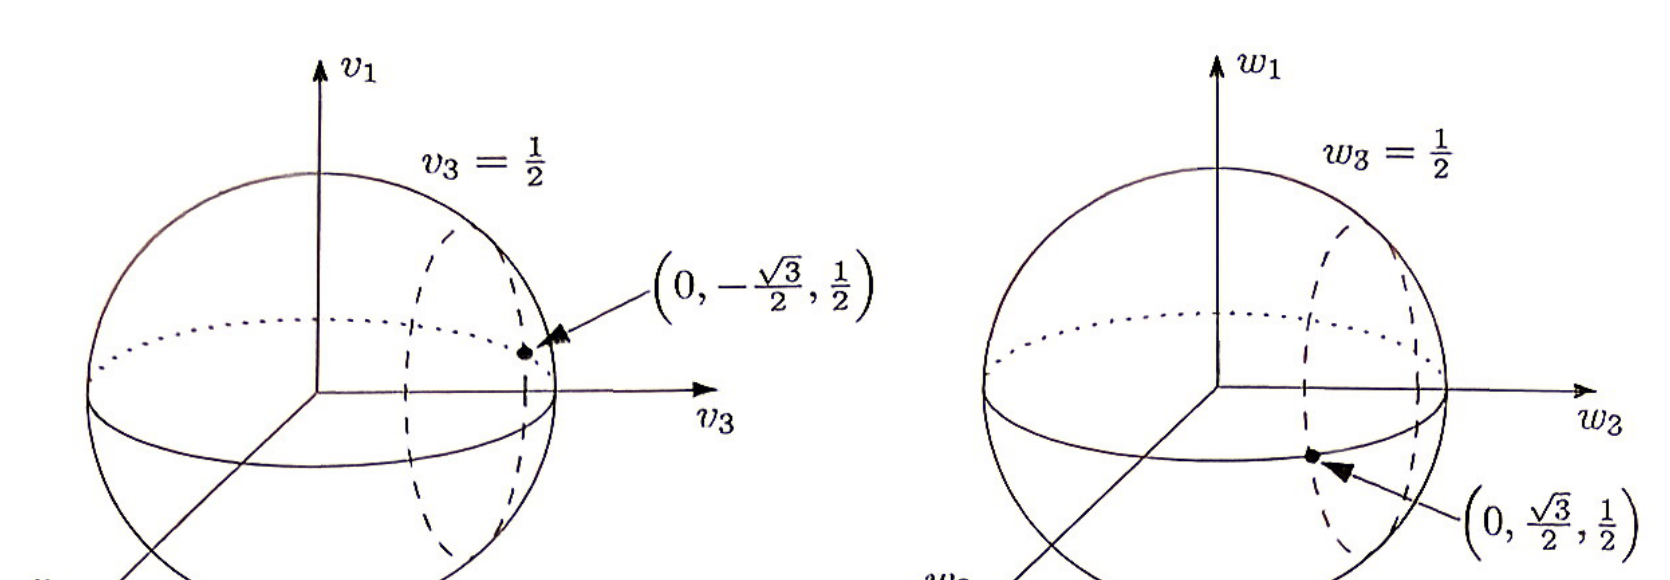
\includegraphics[width=0.8\linewidth]{figures/fig_p243_1.png}
  \caption*{图 9.1\quad $S^2\times S^2$ 中 $\{\varphi_G^t(p)\}_{t\in\R/2\pi\Z}$ 的轨道
  （原书 p.235, Figure 9.1；PDF p.243）}
\end{figure}

为简单起见，把这条曲线记作 $C$。于是由注 9.1.2，环面 $\mathbb{T}_{\mathrm{EP}}$ 是
圆周作用 $\{\varphi_F^s\}_{s\in\R/2\pi\Z}$（见注 9.1.1）在曲线 $C$ 上的像，该作用
定义为
\begin{equation*}
  \R/2\pi\Z\cdot(v,w):=\Bigl(
  \begin{pmatrix}1&0&0\\0&\cos(s)&-\sin(s)\\0&\sin(s)&\cos(s)\end{pmatrix}v,\,
  \begin{pmatrix}1&0&0\\0&\cos(s)&-\sin(s)\\0&\sin(s)&\cos(s)\end{pmatrix}w\Bigr)
\end{equation*}
对任意 $(v,w)\in C$ 成立。记矩阵
\begin{equation}\tag{9.8}
  R_s:=\begin{pmatrix}1&0&0\\0&\cos(s)&-\sin(s)\\0&\sin(s)&\cos(s)\end{pmatrix}.
\end{equation}
这个矩阵 $R_s$ 对于我们下面构造第三个环面至关重要。

\textbf{环面三：}考虑 $\C$ 中以 $\sqrt2$ 为半径的标准二维圆盘 $B^2(2)$，其中 $B^2(2)$
由 (1.13) 定义。为在 $S^2\times S^2$ 中得到一个环面，我们按如下三步进行。
\begin{enumerate}[label=(\roman*)]
  \item 取一条（事实上可任取）闭曲线
    $\Gamma\subset\bigl(B^2(2)\cap\{\operatorname{im}(z)>0\}\bigr)$，它围出的区域面积
    等于 $\pi/2$（见图 9.2）。
  \item 经由由下式定义的球极投影
    \begin{equation*}
      \psi(re^{\ii\theta})
      =\Bigl(1-r^2,\ r\cos(\theta)\sqrt{2-r^2},\ r\sin(\theta)\sqrt{2-r^2}\Bigr)
    \end{equation*}
    把 $(B^2(2),\omega_{\mathrm{std}})$ 嵌入到
    $\bigl(S^2,\tfrac12\omega_{\mathrm{area}}\bigr)$ 中，
% >>> p244
    其中 $re^{\ii\theta}\in B^2(\sqrt2)$。注意该映射关于
    $\tfrac12\omega_{\mathrm{area}}$ 是辛同胚。
  \item 记 $\Delta_\Gamma$ 为对角集
    $\{(x,x)\in B^2(2)\times B^2(2)\mid x\in\Gamma\}$。然后考虑如下圆周作用在曲线
    $(\psi,\psi)(\Delta_\Gamma)\subset S^2\times S^2$ 上产生的扭转旋转：
    \begin{equation*}
      \R/2\pi\Z\cdot(v,w):=(R_sv,\,R_{-s}w),
    \end{equation*}
    其中 $(v,w)\in(\psi,\psi)(\Delta_\Gamma)$，$R_s$ 由 (9.8) 定义。可以证明这个
    圆周作用的像是 $S^2\times S^2$ 中的拉格朗日环面，记作
    $\mathbb{T}_{\mathrm{CS}}$。这类拉格朗日环面最早由 Y. Chekanov 与 F. Schlenk
    在 [48] 中引入。
\end{enumerate}
% [Tutor Note: 原文疑误/记号含混——本段先说 $B^2(2)$ 「半径为 $\sqrt2$」，随后又写
% $re^{\ii\theta}\in B^2(\sqrt2)$，两种记号不一致；按上下文 $B^2(2)$ 应指半径
% $\sqrt2$ 的圆盘（其面积为 $2\pi$，恰等于 $(S^2,\tfrac12\omega_{S^2})$ 的总面积），
% 故 $(B^2(2),\omega_{\mathrm{std}})$ 与 $(S^2,\tfrac12\omega_{\mathrm{area}})$ 的
% 辛同胚是等面积的。译文按原文照译，详见 qsg/notes/review_ch09a.md。另外原文 "via the
% stereographic projection define by" 中 define 应为 defined。]

\begin{figure}[htbp]
  \centering
  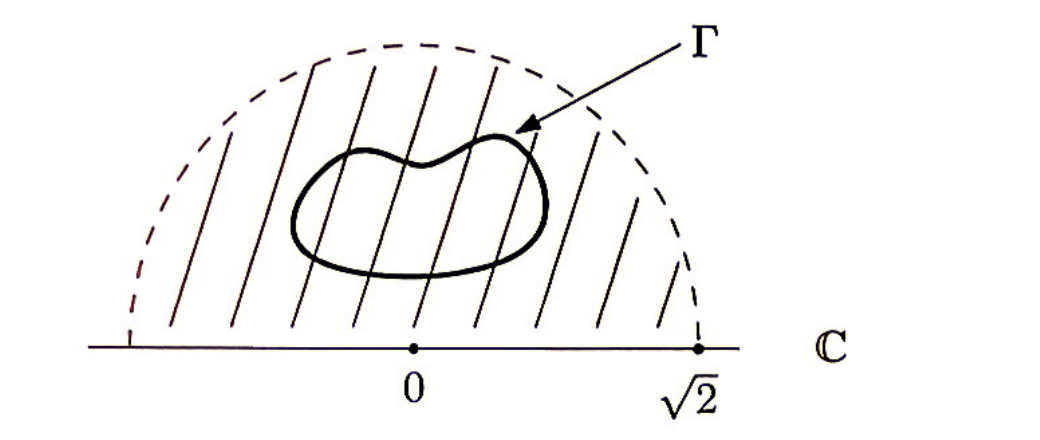
\includegraphics[width=0.6\linewidth]{figures/fig_p243_2.png}
  \caption*{图 9.2\quad 半圆盘内的一条闭曲线 $\Gamma$（原书 p.235, Figure 9.2；
  PDF p.243）}
\end{figure}

有趣的是，环面 $\mathbb{T}_{\mathrm{EP}}$ 与 $\mathbb{T}_{\mathrm{CS}}$ 在相差一个
辛同胚的意义下是相同的。

\begin{wthm}{9.1.1}（[170] 中的命题 2.4）
  上述定义的 $\mathbb{T}_{\mathrm{EP}}$ 与 $\mathbb{T}_{\mathrm{CS}}$ 在
  $\bigl(S^2\times S^2,\pi_1^*(\tfrac12\omega_{\mathrm{area}})
  +\pi_2^*(\tfrac12\omega_{\mathrm{area}})\bigr)$ 中辛同构。
\end{wthm}

\begin{wproof}
  这里我们给出证明的梗概（其中要点 (a) 基于 A. Gadbled 在 [91] 中的一个巧妙观察），
  细节留给有兴趣的读者。证明主要基于以下三条观察。
  \begin{enumerate}[label=(\alph*)]
    \item 我们有如下关系：
    \begin{equation}\tag{9.9}
    \begin{aligned}
      &\Bigl(\begin{pmatrix}1&0&0\\0&1&0\\0&0&1\end{pmatrix},
      \begin{pmatrix}-1&0&0\\0&-1&0\\0&0&1\end{pmatrix}\Bigr)(R_s,R_s)\\
      &\qquad=\bigl(R_s,R_{-s}\bigr)
      \Bigl(\begin{pmatrix}1&0&0\\0&1&0\\0&0&1\end{pmatrix},
      \begin{pmatrix}-1&0&0\\0&-1&0\\0&0&1\end{pmatrix}\Bigr).
    \end{aligned}
    \end{equation}
    \item 在构造中，环面 $\mathbb{T}_{\mathrm{CS}}$ 实际上（在相差一个辛同胚的
      意义下）不依赖于 $B^2(2)\cap\{\operatorname{im}(z)>0\}$ 中的曲线 $\Gamma$，
      只要它围出的面积为 $\pi/2$。
    \item 由如下线性映射作用，是 $S^2\times S^2$ 上的辛同胚：
    \begin{equation}\tag{9.10}
      A:=\Bigl(\begin{pmatrix}1&0&0\\0&1&0\\0&0&1\end{pmatrix},
      \begin{pmatrix}-1&0&0\\0&-1&0\\0&0&1\end{pmatrix}\Bigr).
    \end{equation}
  \end{enumerate}
  由练习 9.1.2 正下方的那段文字以及上面的 (c) 可知，(9.9) 的第一行恰好等于
  $\mathbb{T}_{\mathrm{EP}}$ 经 (9.10) 中辛同胚 $A$ 作用后的像。又容易验证，
  $A(C)$ 作为 $B^2(2)\times B^2(2)$ 中的曲线围出的区域面积为 $\pi/2$。因此由上面的
  (b)，(9.9) 的右端与 $\mathbb{T}_{\mathrm{CS}}$ 辛同胚。所以
  $\mathbb{T}_{\mathrm{CS}}\simeq\mathbb{T}_{\mathrm{EP}}$。
\end{wproof}
% [Tutor Note: 易错预警——(9.9) 中第二个矩阵是 $\operatorname{diag}(-1,-1,1)$；
% 直接计算可见 $D R_s=R_{-s}D$ 当且仅当 $D=\operatorname{diag}(d_1,d_2,d_3)$ 满足
% $d_3=-d_2$，而 $(d_1,d_2,d_3)=(-1,-1,1)$ 正满足此条件（$d_1$ 任意）。若误写成
% $\operatorname{diag}(1,-1,1)$，则 $D R_s\neq R_{-s}D$，(9.9) 不成立。另注意 $A$
% 在第二个 $S^2$ 因子上的线性映射保持 $S^2$（因为它是正交矩阵）且保持其面积形式。]

与此相反，我们有如下结果。

% >>> p245
\begin{wthm}{9.1.2}
  Clifford 环面 $\mathbb{T}_{\mathrm{Clifford}}$ 与 $\mathbb{T}_{\mathrm{EP}}$ 不
  辛同构（从而也不与 $\mathbb{T}_{\mathrm{CS}}$ 辛同构）。
\end{wthm}

为证明上述定理，我们需要某种辛不变量，它将由一种称为 $A_\infty$-代数的高级代数结构
构造出来，该结构将在下一节介绍。
